\documentclass[tikz,border=2]{standalone}
\usetikzlibrary{shadows,arrows,shapes,positioning,calc,backgrounds,fit}
% Define the layers to draw the diagram
%
\newcommand{\vanish}[1]{}
%\newcommand{\vanish}[1]{#1}
\begin{document}
\pgfdeclarelayer{bg}
\pgfdeclarelayer{fg}
\pgfsetlayers{bg,main,fg}
%
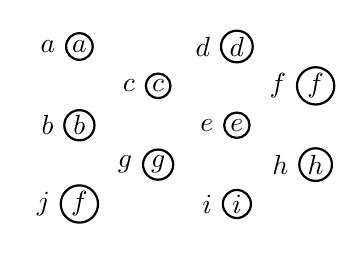
\begin{tikzpicture}
[node distance=1cm,
bend angle=20,
subdue/.style={draw=black!15},
every fit/.style={fill=black!20,ellipse},
%
node/.style={shape=circle,draw=black,thick, inner sep = 1pt},
group1/.style={shape=circle,draw=black,thick},
group2/.style={shape=circle,draw=black},
group3/.style={shape=circle,draw=black},
group4/.style={shape=circle,draw=black},
ignored/.style={shape=circle,subdue,inner sep=2pt},
seed/.style={vertex,fill=red},
infected/.style={vertex,fill=brown},
%
myedge/.style={semithick,subdue},
dedge/.style={>=latex', shorten >=.1pt, shorten <=.1pt, semithick}]

\node (a) [node,label=left:$a$] at (0,0) {$a$};
\node (b) [node,label=left:$b$] at (0,-1) {$b$};
\node (c) [node,label=left:$c$] at (1,-.5) {$c$};
\node (d) [node,label=left:$d$] at (2,0) {$d$};
\node (e) [node,label=left:$e$] at (2,-1) {$e$};
\node (f) [node,label=left:$f$] at (3,-.5) {$f$};
\node (g) [node,label=left:$g$] at (1,-1.5) {$g$};
\node (h) [node,label=left:$h$] at (3,-1.5) {$h$};
\node (i) [node,label=left:$i$] at (2,-2) {$i$};
\node (j) [node,label=left:$j$] at (0,-2) {$f$};

\end{tikzpicture}
\end{document}

\node (a11) [ignored] at (1.2,-0.3){\vanish{11}};
\node (a12) [ignored] at (1.2,-.7){\vanish{12}};

\node (a3) [infected] at (-.8,-2){\vanish{3}};
\node (a14) [vertex] at (-.1,-1.7){\vanish{14}};
\node (a15) [seed] at (-.2,-2.7){\vanish{15}};

\node (a4) [vertex] at (.5,-3){\vanish{4}};
\node (a16) [vertex] at (0.3,-3.4){\vanish{16}};
\node (a17) [vertex] at (0.7,-3.4){\vanish{17}};

\node (a5) [infected] at (.3,-1.3){\vanish{5}};
\node (a6) [vertex] at (.7,-2.2){\vanish{6}};
\node (a7) [ignored] at (1,-1.3){\vanish{7}};
\node (a8) [ignored] at (1.5,-2){\vanish{8}};

\node (a13) [ignored] at (2,-1.8){\vanish{13}};
\node (a18) [ignored] at (1.8,-2.5){\vanish{18}};
\node (a19) [ignored] at (2,-2.2){\vanish{19}};
\node at (-.5,.5) {$H_{LT}$};
\node at (2.1,0.2) {\parbox{1.5cm}{\small Tree with a directed cycle}};


\draw[dedge,<-] (a1) -- (a2);
\draw[dedge,->] (a1) -- (a5);
\draw[dedge,->] (a1) -- (a9);
\draw[myedge] (a1) -- (a10);

\draw[myedge] (a2) -- (a3);
\draw[dedge,<-] (a2) -- (a5);
\draw[myedge] (a2) -- (a14);

%\draw[myedge] (a3) -- (a4);
%\draw[myedge] (a3) -- (a6);
\draw[dedge,<-] (a3) to (a15);

\draw[dedge,->] (a4) -- (a6);
\draw[dedge,->] (a4) -- (a15);
\draw[dedge,<-] (a4) -- (a14);
\draw[dedge,->] (a4) -- (a16);
\draw[dedge,->] (a4) -- (a17);

\draw[myedge] (a5) -- (a6);
\draw[myedge] (a5) -- (a7);
%\draw[myedge] (a5) -- (a8);
%\draw[myedge] (a5) -- (a10);
%\draw[myedge] (a5) -- (a14);

\draw[myedge] (a6) -- (a7);
\draw[myedge] (a6) -- (a8);
\draw[dedge,->] (a6) -- (a14);

\draw[myedge] (a7) -- (a8);
\draw[myedge] (a7) to (a10);
%\draw[dedge,->,out=90,in=-45] (a7) to (a10);
%\draw[dedge,<-,out=135,in=-90] (a7) to (a10);
\draw[myedge] (a7) -- (a14);

\draw[myedge] (a8) -- (a13);
\draw[myedge] (a8) -- (a18);
\draw[myedge] (a8) to (a19);

\draw[myedge] (a10) -- (a11);
\draw[myedge] (a10) -- (a12);

\begin{pgfonlayer}{bg}
\node[inner sep=-3pt,fit=(a1)(a2)(a5)(a9),rotate=-35] at ($(a1)+(0.3,-.45)$) {};
\end{pgfonlayer}


%\node (a3) [vertex,below right=of v11,label=right:$3$] {\vanish{}};
%\node (a4) [vertex,below=of v21,label=left:$4$] {};
%\node (a5) [vertex,below=of v31,label=right:$5$] {};
%\node (a6) [vertex,below=of v41,label=left:$6$] {};
%\node (a7) [vertex,below=of v51,label=right:$7$] {};
%\draw[myedge] (v11) -- (v21) -- (v31) -- (v51) -- (v41) -- (v61) -- (v71)
%-- (v51);
%\draw[myedge] (v11) -- (v31);
%\draw[myedge] (v21) -- (v41);
%
%\node (v12) [vertex,label=above:$1$,fill] at (4,0) {};
%\node (v22) [vertex,below left=of v12,label=left:$2$] {};
%\node (v32) [vertex,below right=of v12,label=right:$3$] {};
%\node (v42) [vertex,below=of v22,label=left:$4$] {};
%\node (v52) [vertex,below=of v32,label=right:$5$] {};
%\node (v62) [vertex,below=of v42,label=left:$6$,fill] {};
%\node (v72) [vertex,below=of v52,label=right:$7$] {};
%\draw[dedge,<-] (v12) -- (v22);
%\draw[dedge,<-] (v32) -- (v12);
%\draw[dedge,<-] (v22) -- (v32);
%\draw[dedge,<-] (v42) -- (v22);
%\draw[dedge,<-] (v52) -- (v32);
%
%\draw[dedge,<-] (v62) [out=45,in=135] to (v72);
%\draw[dedge,->] (v62) [out=-45,in=-135] to (v72);

\end{tikzpicture}
{}
\end{document}
